


\begin{exercice}[]
Compléter le tableau suivant.

\begin{center}
\begin{Ltableau}{\linewidth}{4}{c}
\hline
\textbf{Corps étudié} & \textbf{Receveur} & \textbf{Acteur} & \textbf{Type d'action}  \\ \hline
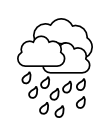
\includegraphics[angle=0,width=.7cm]{nuagePluie} & Goutte &  &  \\ \hline
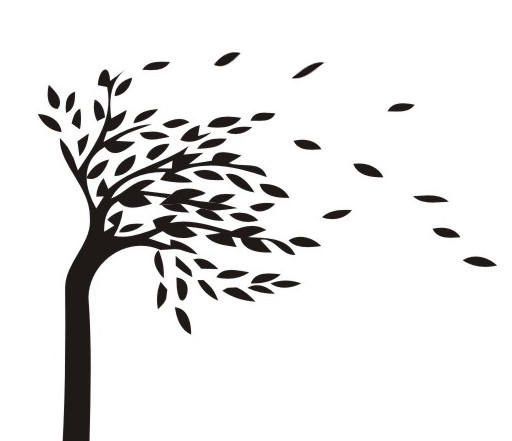
\includegraphics[angle=0,width=1.2cm]{tree} & Feuille & & \\ \hline
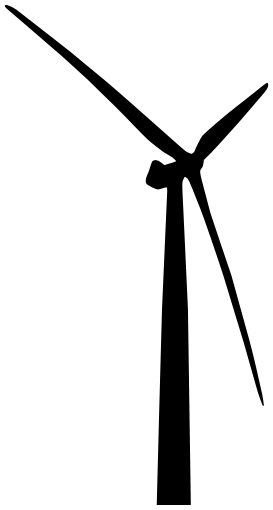
\includegraphics[angle=0,width=.7cm]{eolienne} & Pâle & & \\ \hline
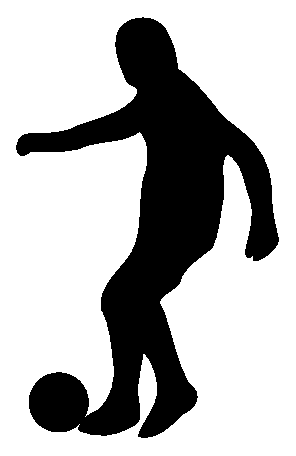
\includegraphics[angle=0,width=.7cm]{footballer} & Ballon & & \\ \hline
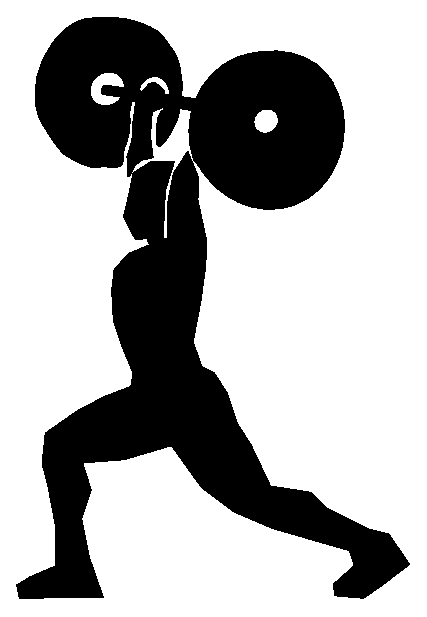
\includegraphics[angle=0,width=.7cm]{halterophile} & Homme & & \\ \hline
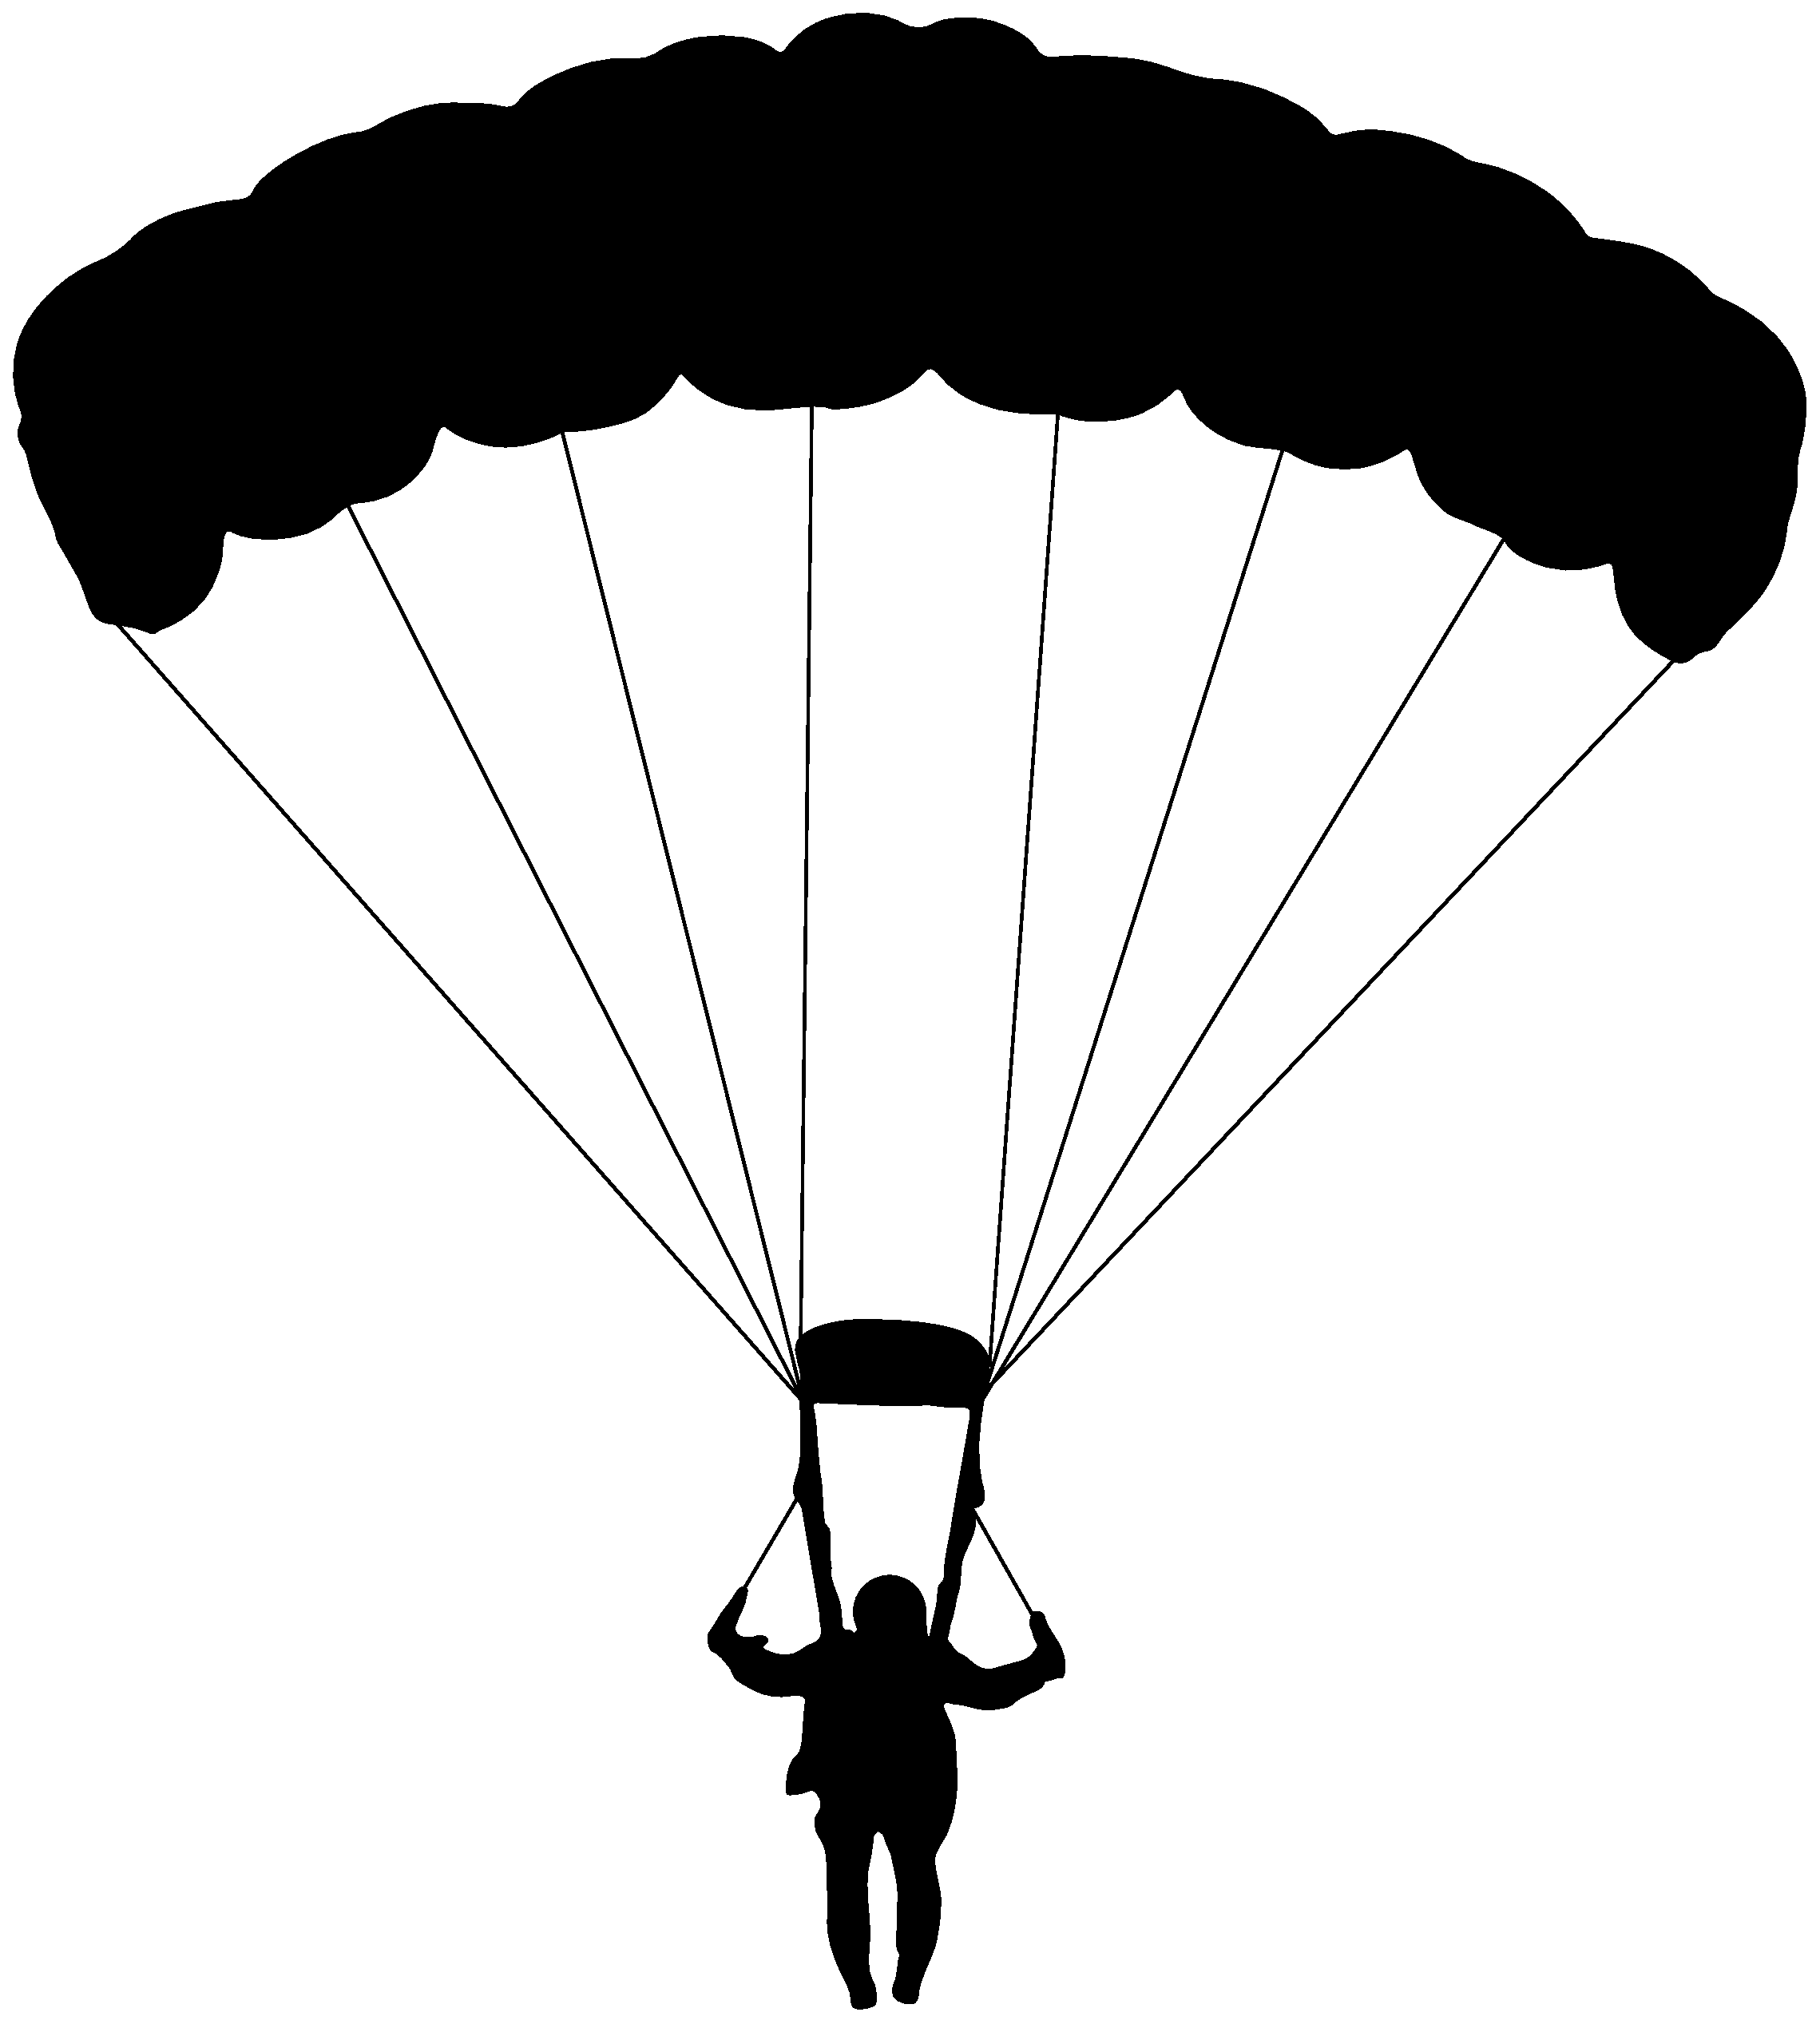
\includegraphics[angle=0,width=1.2cm]{parachute} & Homme & &  \\ \hline
\end{Ltableau}
\end{center}

\end{exercice}

\begin{corrige}
Acteur et receveur

\begin{center}
\begin{Ltableau}{\linewidth}{4}{c}
\hline
\textbf{Corps étudié} & \textbf{Receveur} & \textbf{Acteur} & \textbf{Type d'action}  \\ \hline
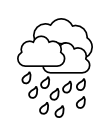
\includegraphics[angle=0,width=.4cm]{nuagePluie} & Goutte & Terre & Distance  \\ \hline
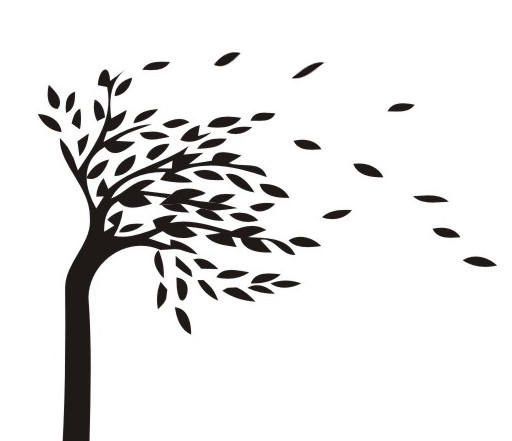
\includegraphics[angle=0,width=.7cm]{tree} & Feuille & Air & Contact \\ \hline
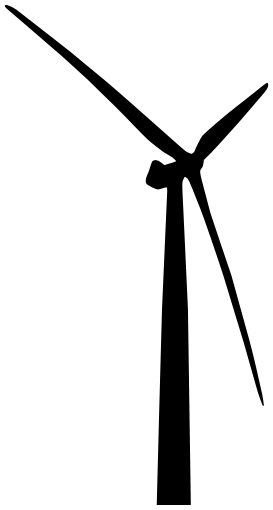
\includegraphics[angle=0,width=.4cm]{eolienne} & Pâle & Air & Contact \\ \hline
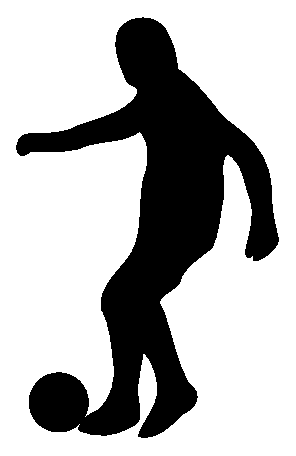
\includegraphics[angle=0,width=.4cm]{footballer} & Ballon & Joueur & Contact \\ \hline
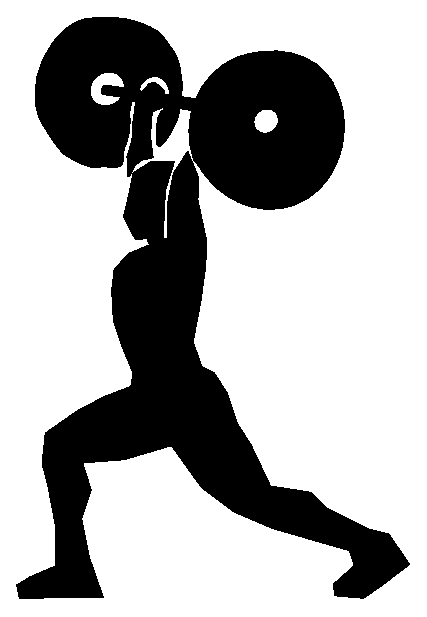
\includegraphics[angle=0,width=.4cm]{halterophile} & Homme & Haltères & Contact \\ \hline
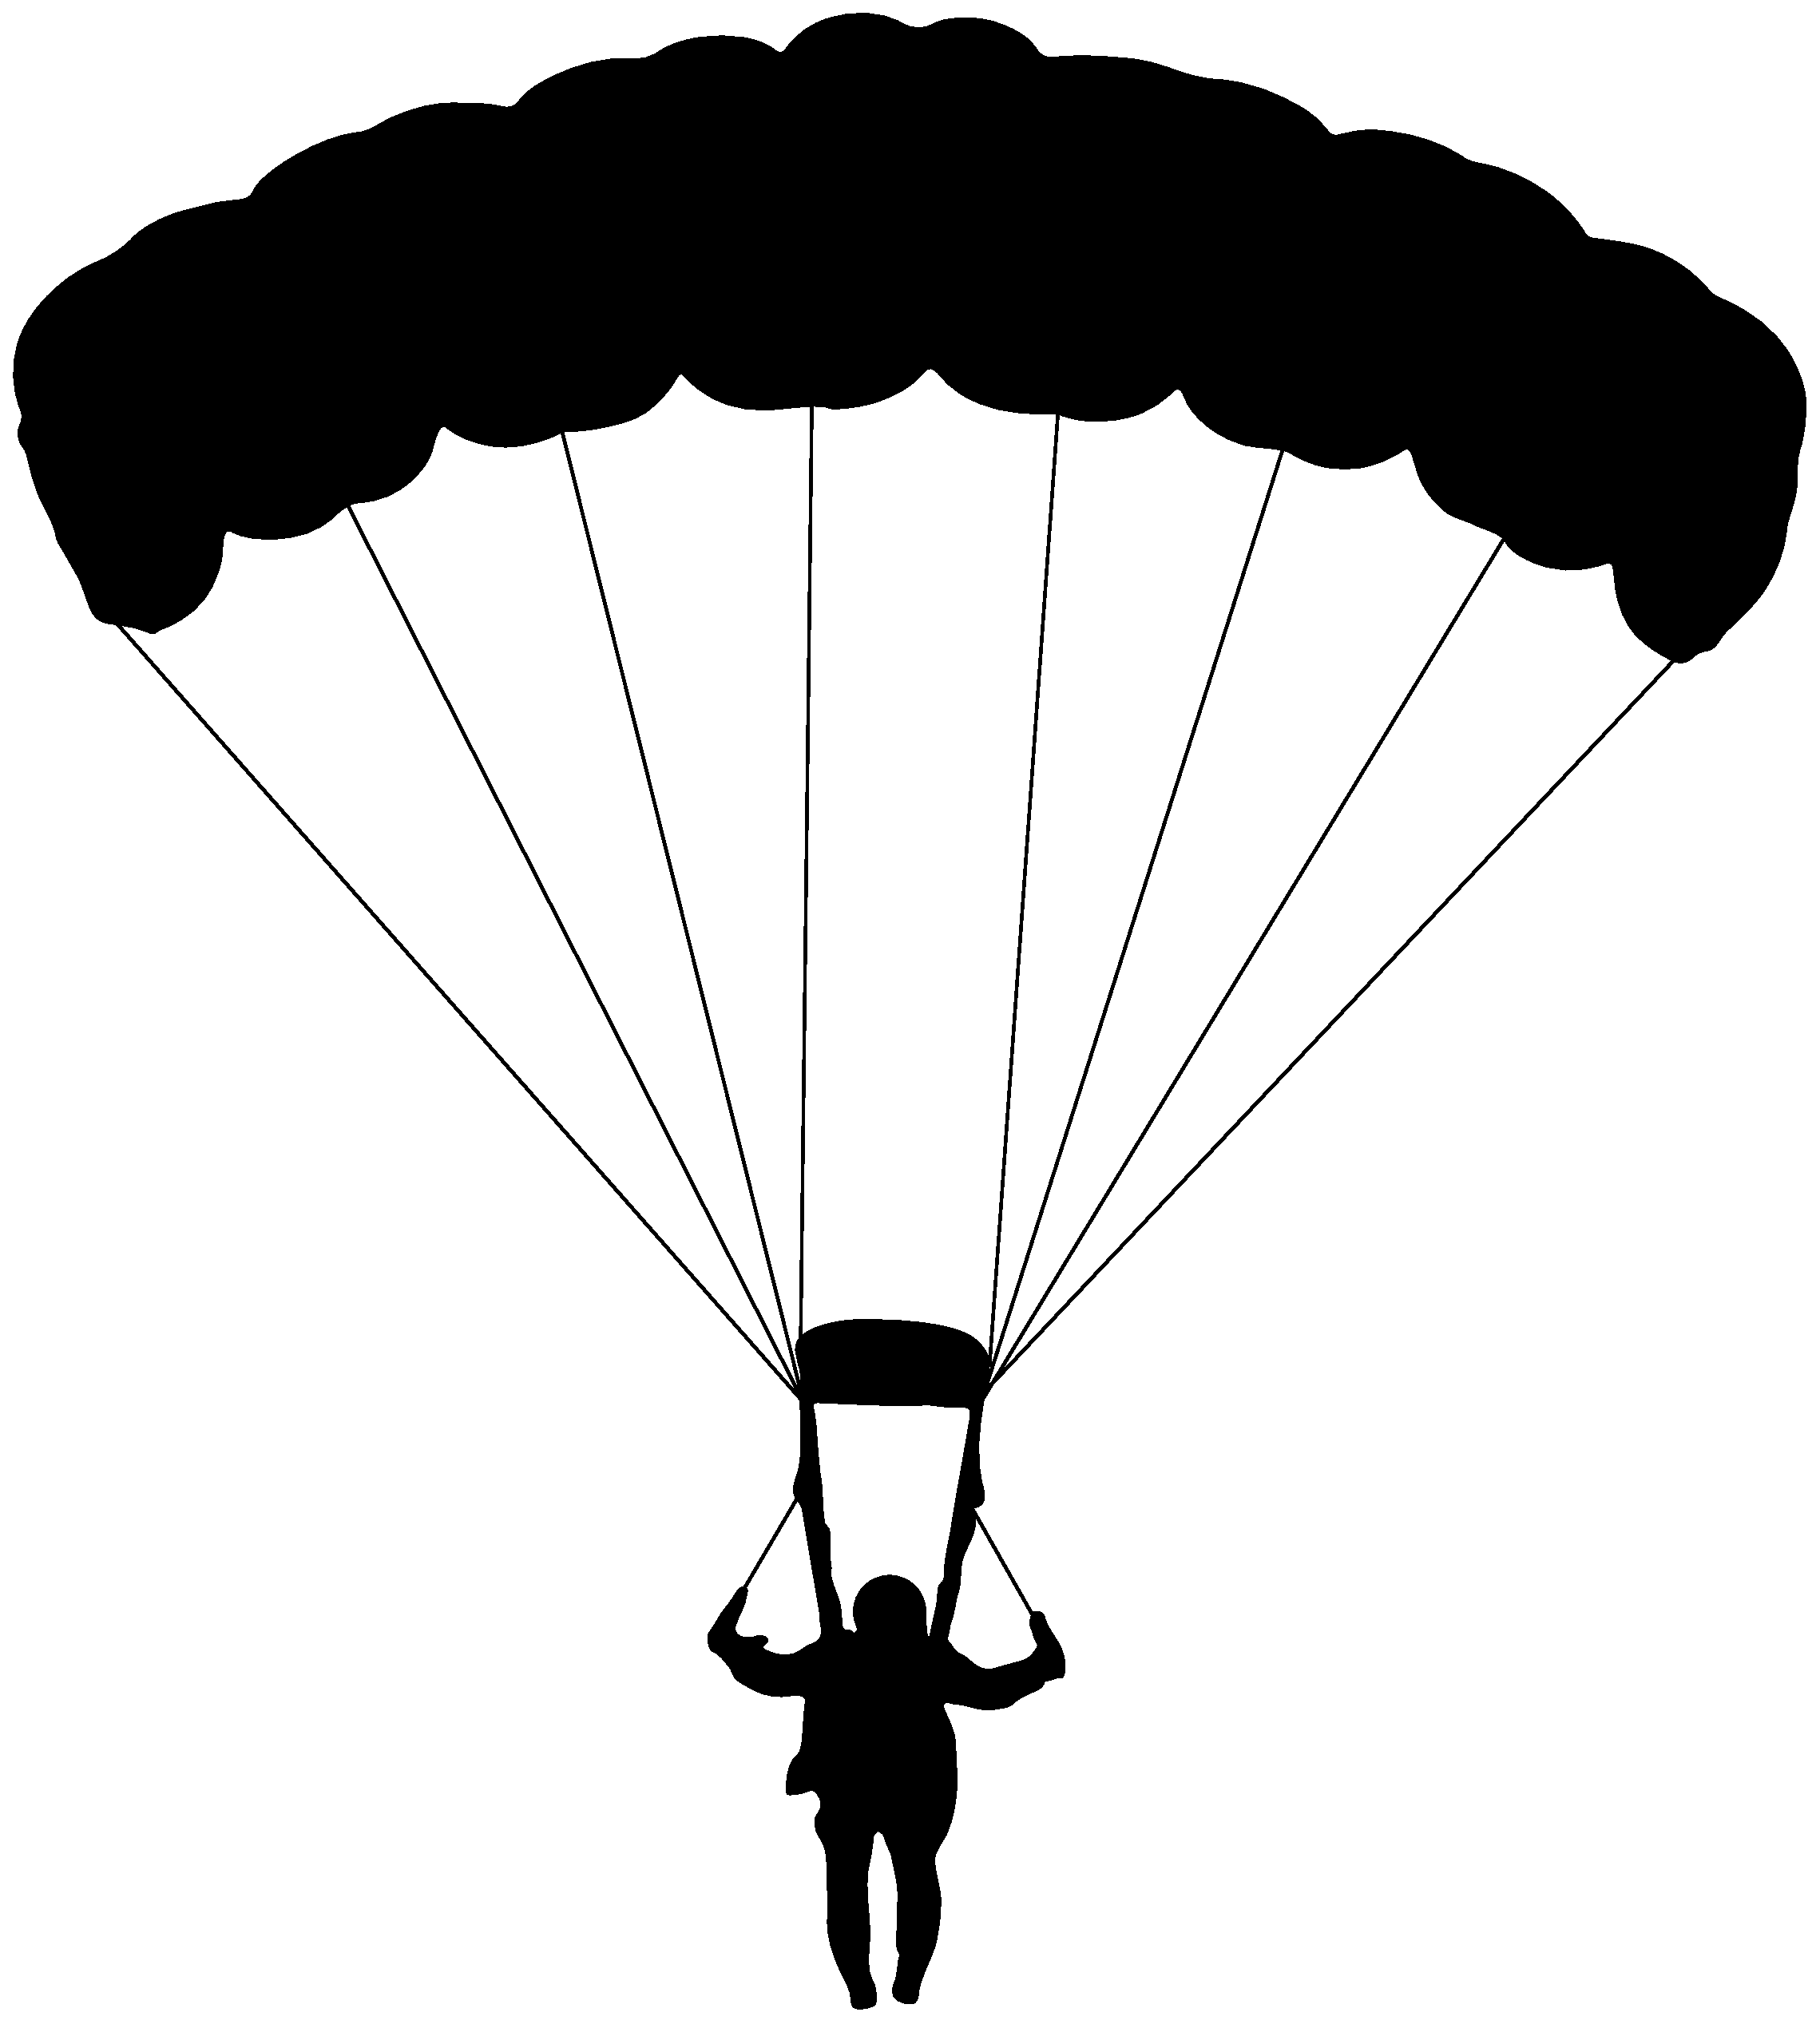
\includegraphics[angle=0,width=.7cm]{parachute} & Homme & Parachute & Contact \\ \hline
\end{Ltableau}
\end{center}

\end{corrige}



\begin{exercice}[]\ExerciceRefMethode{methodeForceEchelle}
\label{representeVecteur}

Une personne tire un objet par l'intermédiaire d'une corde. On s'intéresse à la force exercée par la corde sur l'objet. Elle a pour valeur 3\,N.

\vspace{1em}
\begin{center}
    \includegraphics[width=.4\linewidth]{./objetMain}   
\end{center}

\begin{enumerate}
\item Donner toutes les caractéristiques de la force.
\item On prend comme échelle 1\,cm représente 1\,N. Calculer la longueur de la flèche utilisée pour représenter la force.  
\item Représenter, à l'échelle, la force sur le schéma.
\end{enumerate}


\end{exercice}

%\begin{corrige}

%\end{corrige}


% fin de l'exercice


\begin{exercice}
Anaïs tire sur le tendeur avec sa main. Représenter la force exercée par la main ($M$) sur le tendeur ($T$), sachant qu'elle a pour valeur 5\,N. Échelle : 1\,cm pour 2\,N.  

\vspace{1em}
\begin{center}
    \includegraphics[width=.4\linewidth]{./tendeurMain}   
\end{center}

\end{exercice}

%\begin{corrige}
%Tendeur et main

%\end{corrige}





\begin{exercice}
Au service, la force $\vect{F_1}$ exercée par la raquette d'un joueur de tennis sur la balle vaut 1200\,N. Sur le schéma, on a représenté en pointillé la ligne d'action des forces. Représenter $\vect{F_1}$ à l'échelle 1\,cm pour 500\,N.

\vspace{1em}
\begin{center}
    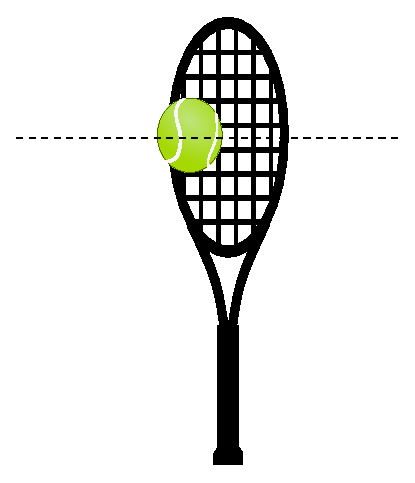
\includegraphics[width=.4\linewidth]{./tennisBall}   
\end{center}

\end{exercice}

%\begin{corrige}
%Service au tennis

%\end{corrige}


















\begin{exercice}
Répondre aux questions suivantes sur les forces.
\begin{enumerate}
\item Avec quel appareil mesure-t-on l'intensité d'une force ?
\item Quelle est l'unité légale de force ?
\item Quel est son symbole ?
\end{enumerate}
\end{exercice}


\begin{corrige}
\begin{enumerate}
\item L'intensité d'une force se mesure grâce à un dynamomètre.
\item L'unité légale de la force est le newton.
\item Symbole du newton : N.
\end{enumerate}
\end{corrige}






\begin{exercice}
Répondre aux questions suivantes sur les forces.
\begin{enumerate}
\item Que modélisent les forces ? 
\item Quelles sont les quatre caractéristiques d'une force ?
\item Par quoi est représentée une force ?
\end{enumerate}
\end{exercice}


\begin{corrige}
\begin{enumerate}
\item Les forces modélisent des actions mécaniques.
\item Les quatre caractéristiques sont : droite d'action (direction), sens, intensité, point d'application.
\item Une force est représentée par un vecteur.
\end{enumerate}
\end{corrige}






\begin{exercice}
Dire si les propositions suivantes sont vraies ou fausses. Corriger celles qui sont fausses.
\begin{enumerate}
\item Les actions de contact peuvent être ponctuelles ou réparties.
\item L'action du vent sur la voile du véliplanchiste est une action à distance.
\item L'unité légale de la force est le kilogramme, de symbole kg.
\item La valeur d’une force se mesure avec un dynamomètre.
\end{enumerate}
\end{exercice}


\begin{corrige}
\begin{enumerate}
\item Vrai 
\item Faux (contact entre l'air et la voile)
\item Faux, c'est le newton (N).
\item Vrai
\end{enumerate}
\end{corrige}








\begin{exercice}
Observer la figure ci-dessous.

\begin{minipage}[c]{.28\linewidth}
\centering
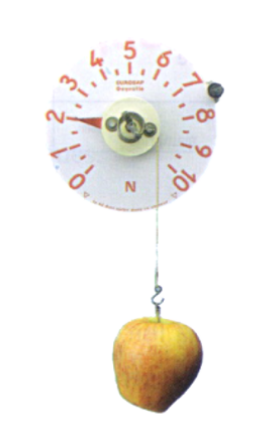
\includegraphics[width=.8\linewidth]{pommeDynamo}
\end{minipage}\hfill%
\begin{minipage}[c]{.68\linewidth}
\begin{enumerate}
\item Quel est le nom de l'appareil de mesure ?
\item En quelle unité est-il gradué ?
\item Quelle est la valeur de la force ? 
\end{enumerate}
\end{minipage}
\end{exercice}


\begin{corrige}
\begin{enumerate}
\item L'appareil est un dynamomètre.
\item Il est gradué en newton.
\item Par lecture graphique, on trouve $F=2$\,N. 
\end{enumerate}
\end{corrige}








\begin{exercice}
Indiquer si les actions mécaniques suivantes sont des actions de contact ou des actions à distance :
\begin{enumerate}
\item action du marteau sur le clou ;
\item action du pied sur le ballon ;
\item action de l'aimant sur la bille de fer ;
\item action du vent sur le cerf-volant ;
\item action de la Lune sur les océans.
\end{enumerate}
\end{exercice}


\begin{corrige}
\begin{enumerate}
\item Marteau et clou : action de contact.
\item Pied et ballon : action de contact.
\item Aimant et bille : action à distance.
\item Vent et cerf-volant : action de contact.
\item Lune et océan : action à distance.
\end{enumerate}
\end{corrige}















\begin{exercice}
Sachant que l'intensité de la force $\vect{F}$ est de 100\,N, donner toutes les caractéristiques de la force ainsi que l'échelle utilisée pour la représenter.

\vspace{1em}
\begin{center}
    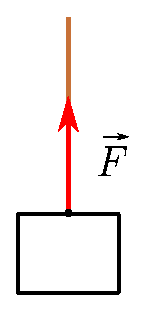
\includegraphics[width=.15\linewidth]{cubeCable}
\end{center}

\end{exercice}


\begin{corrige}
\begin{enumerate}
\item Force : $F$ (tension du fil).
\item Point d'application : jonction entre corde et solide.
\item Droite d'action : la corde.
\item Sens : de bas en haut.
\item Intensité : $F=100$\,N. 
\end{enumerate}
\end{corrige}







\begin{exercice}
Un marteau exerce une force sur un clou. Sachant que l'intensité de la force $\vect{F}$ est de 50\,N, donner toutes les caractéristiques de la force puis la représenter en utilisant l'échelle 1\,cm pour 25\,N.

\vspace{1em}
\begin{center}
    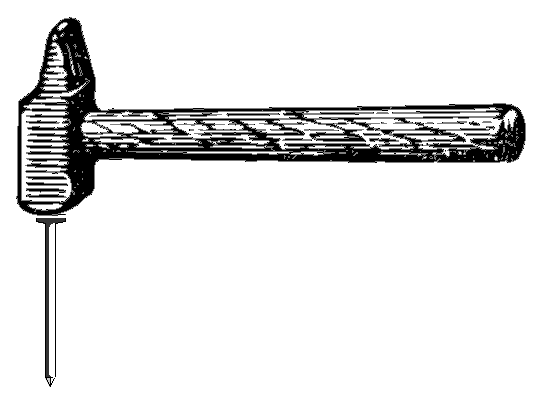
\includegraphics[width=.4\linewidth]{marteauClou}
\end{center}

\end{exercice}


\begin{corrige}
\begin{enumerate}
\item Force : $F$ (appui du marteau sur le clou).
\item Point d'application : tête du clou.
\item Droite d'action : droite matérialisée par le clou.
\item Sens : de haut en bas.
\item Intensité : $F=50$\,N. 
\end{enumerate}

\begin{center}
    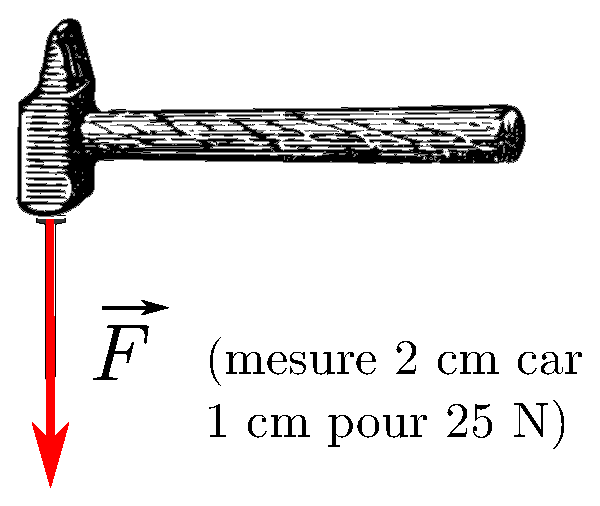
\includegraphics[width=.4\linewidth]{marteauClouCorrection}
\end{center}

\end{corrige}








\begin{exercice}
Une personne pousse un wagonnet comme indiqué sur le schéma ci-dessous, avec une force d'intensité 500\,N. Donner les caractéristiques de la force puis la représenter à l'échelle 1\,cm représente 200\,N.

\vspace{1em}
\begin{center}
    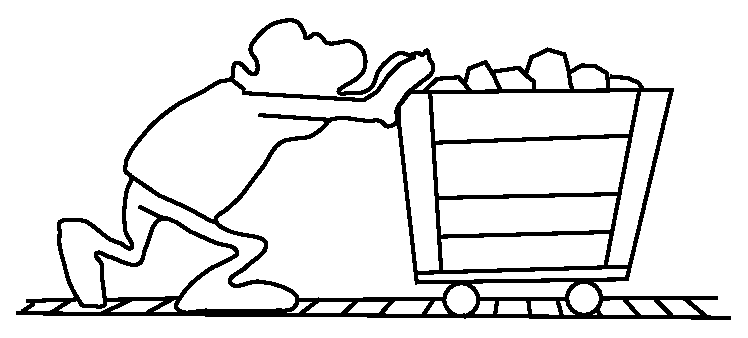
\includegraphics[width=.5\linewidth]{wagonnet}
\end{center}

\end{exercice}


\begin{corrige}
\begin{enumerate}
\item Force : $F$ (action de l'homme sur le wagonnet).
\item Point d'application : point de contact main--wagonnet.
\item Droite d'action : droite parallèle aux rails, passant par les mains.
\item Sens : de l'homme vers le wagonnet.
\item Intensité : $F=500$\,N. 
\end{enumerate}

\vspace{1em}

\begin{center}
   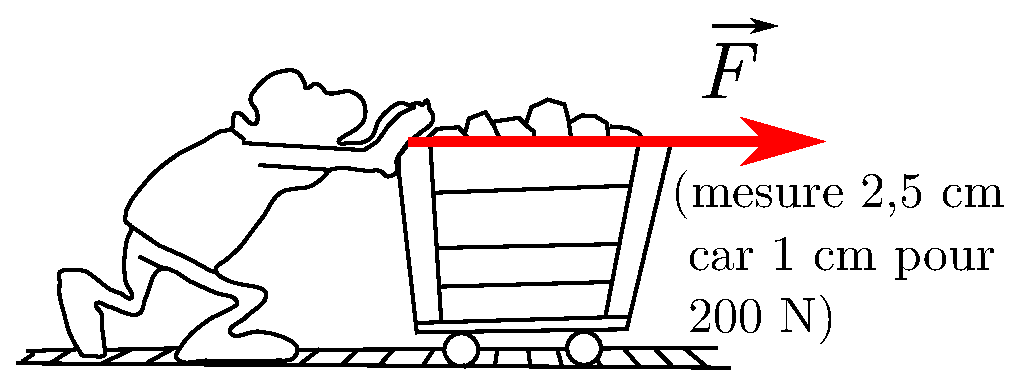
\includegraphics[width=.6\linewidth]{wagonnetCorrection}
 
\end{center}

\end{corrige}


\begin{exercice}\ExerciceRefMethode{methodeAddBoutBout} ou \ExerciceRefMethode{methodeAddParall}
\label{exAddVect}

Pour chacun des cas ci-dessous, indiquer les sommes vectorielles $\vec{a}+\vec{b}$ qui sont correctes et celles qui sont incorrectes.

\vspace{1em}
\begin{center}
    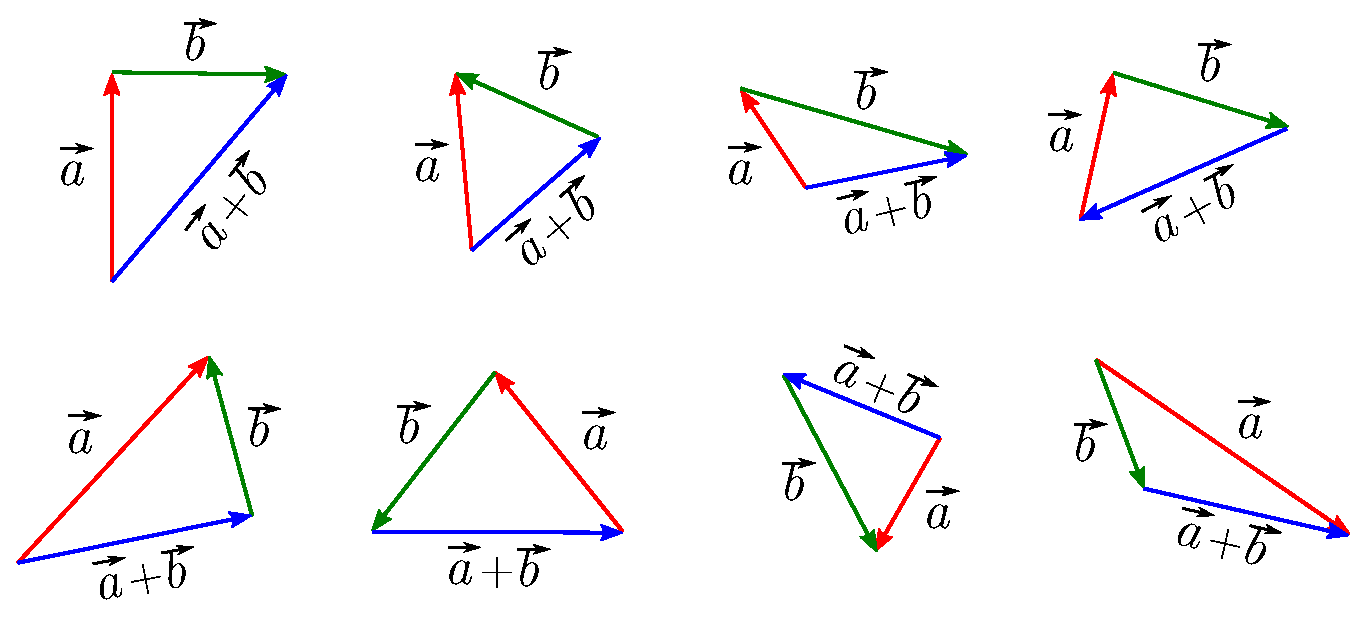
\includegraphics[width=\linewidth]{./sommeVecteurs}   
\end{center}

\end{exercice}





\begin{corrige}
Sommes vectorielles : vrai ou faux ?

\begin{center}
    \includegraphics[width=\linewidth]{./sommeVecteursCorrection}   
\end{center}

\end{corrige}








\begin{exercice}
Pour chacun des cas ci-dessous, tracer graphiquement la somme des deux vecteurs $\vect{a}$ et $\vect{b}$.

\vspace{1em}
\begin{center}
    \includegraphics[width=\linewidth]{./sommeVecteurs2}   
\end{center}

\end{exercice}


\begin{corrige}
Sommes vectorielles

\begin{center}
    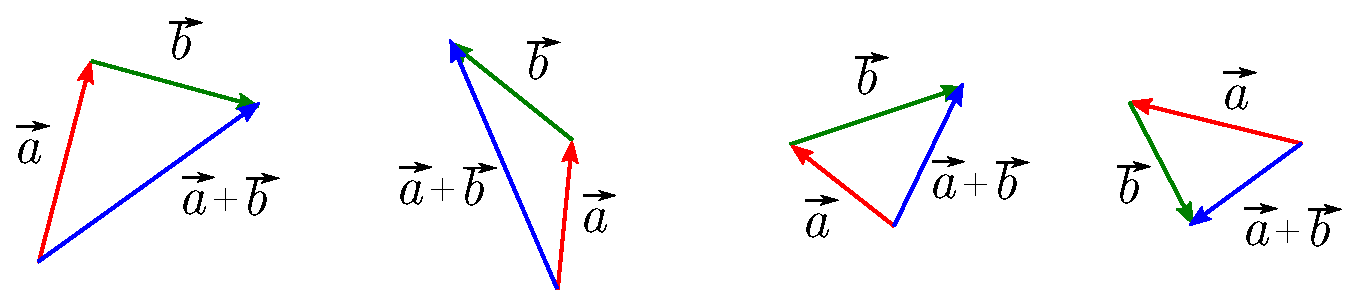
\includegraphics[width=\linewidth]{./sommeVecteurs2Correction}   
\end{center}

\end{corrige}





\begin{exercice}
Dans chacun des cas ci-dessous, un solide est soumis à deux forces $\vec{f_1}$ et $\vec{f_2}$. Tracer à chaque fois la résultante de ces forces, et donner son intensité (échelle : 1\,cm pour 1\,N).

\vspace{1em}
\begin{center}
    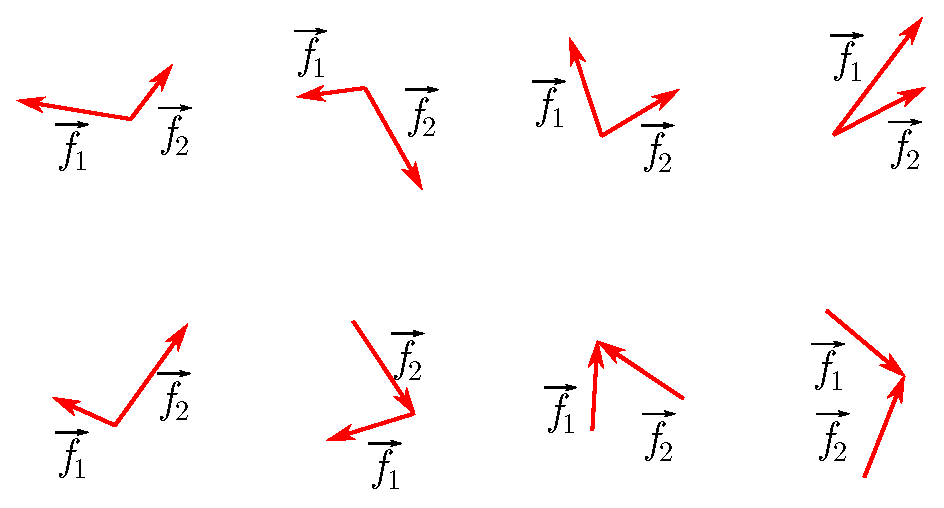
\includegraphics[width=.8\linewidth]{./forcesSolide}   
\end{center}

\end{exercice}


\begin{corrige}
Solide soumis à deux forces

\begin{center}
    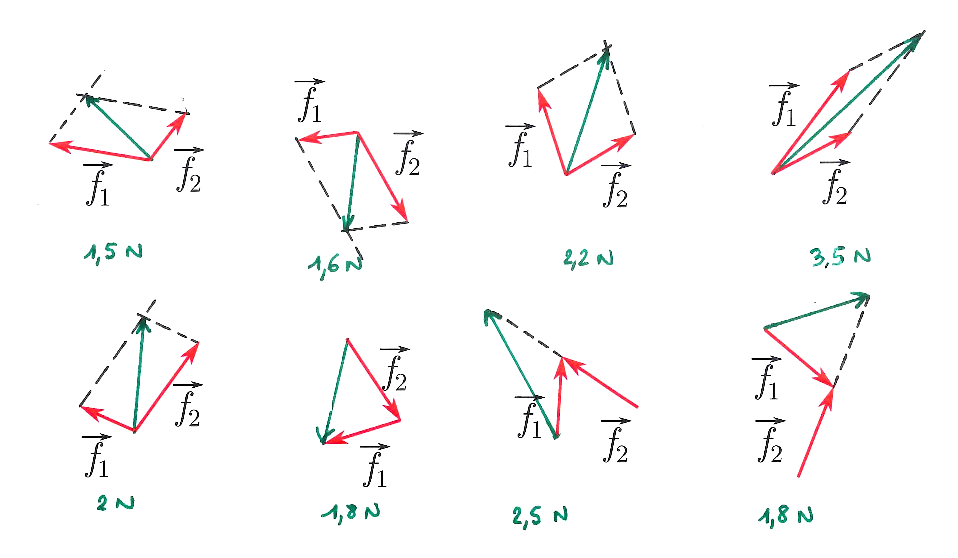
\includegraphics[width=\linewidth]{./forcesSolideCorrection}   
\end{center}

Dans chacun des cas, on mesure la résultante et, en utilisant l'échelle, on obtient l'intensité (indiquée en dessous de chaque figure).
\end{corrige}




\begin{exercice}
Un hors-bord tracte deux skieurs nautiques. Chacun d'eux exerce sur le hors-bord une force de valeur 500\,N.

\vspace{1em}
\begin{center}
    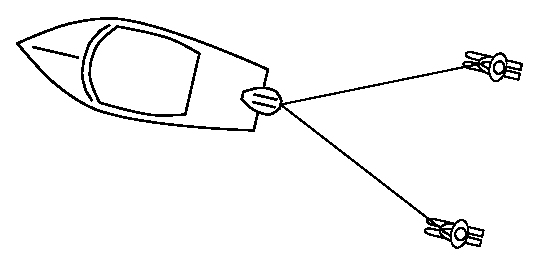
\includegraphics[width=.7\linewidth]{./bateauSki}   
\end{center}


\begin{enumerate}
\item Représenter cette force en utilisant l’échelle 1 cm représente 100 N.
\item Déterminer graphiquement la somme (la résultante) de ces deux forces.
\item Déterminer l'intensité de la résultante.
\end{enumerate}
\end{exercice}


\begin{corrige}
Hors-bord

\begin{center}
    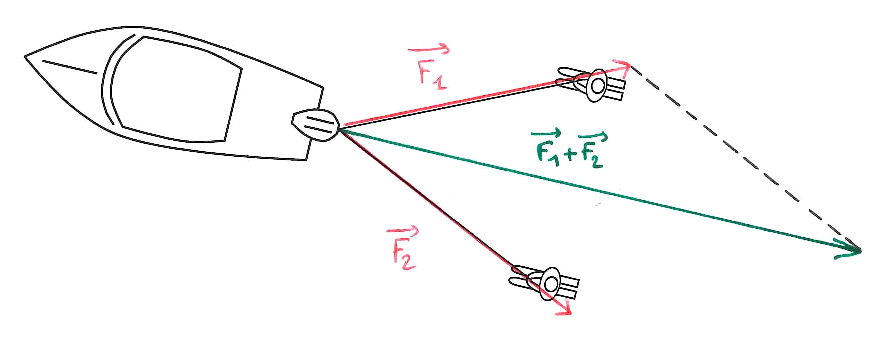
\includegraphics[width=\linewidth]{./bateauSkiCorrection}   
\end{center}

La résultante est mesurée une fois tracée. Elle mesure 9\,cm, soit une intensité de 900\,N (échelle 1\,cm pour 100\,N).    
\end{corrige}





\begin{exercice}
En utilisant deux vecteurs $\vec{u}$ et $\vec{v}$, montrer que $\vec{u} + \vec{v} = \vec{v} + \vec{u}$.
\end{exercice}


\begin{corrige}
Pour cela on trace $\vec{u} + \vec{v}$ puis $\vec{v} + \vec{u}$ :

\vspace{1em}
\begin{center}
    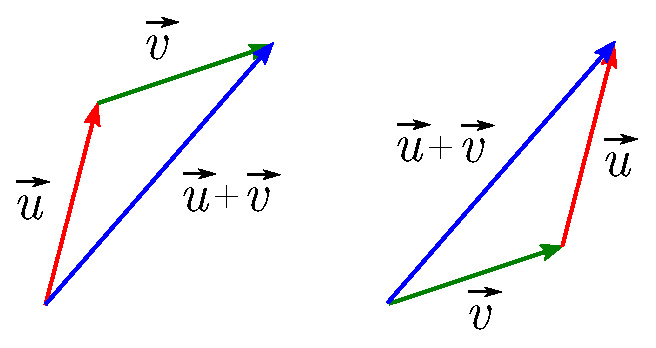
\includegraphics[width=.4\linewidth]{./somme_u_v}   
\end{center}

Graphiquement, on constate que quelque soit l'ordre d'addition, on obtient la même somme vectorielle $\vec{u} + \vec{v}$.
\end{corrige}



\begin{exercice}
Une bille en train de chuter dans l'air est soumise à deux forces (figure ci-dessous).
\vspace{1em}
\begin{center}
    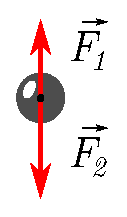
\includegraphics[width=.15\linewidth]{bouleForces}   
\end{center}
%
\begin{enumerate}
\item $\vect{F_1}$ représente une force ; laquelle ?
\item $\vect{F_2}$ représente une force ; laquelle ?
\end{enumerate}

\end{exercice}

\begin{corrige}
\begin{enumerate}
\item $\vect{F_1}$ représente les frottements de l'air qui freinent la bille.
\item $\vect{F_2}$ représente le poids de la bille (dû à la gravité terrestre).
\end{enumerate}
\end{corrige}







\begin{exercice}
Les remorqueurs 1 et 2 tirent une barge, générant une force de tension dans chaque câble $AB$ et $AC$. La tension du câble $AB$ a pour intensité $T_1 = 85$\,kN, celle du câble $AC$, $T_2 = 13$\,kN.
\begin{enumerate}
\item Quelle interaction est modélisée par la force $T_1$ ?
\item Par quel objet est représentée la force $T_1$ ?
\item Donner les caractéristiques de la force de tension $T_1$.
\item Choisir une échelle, tracer au point $A$ la résultante $R$ des forces $T_1$ et $T_2$.
\item Déterminer graphiquement l'intensité de $R$.
\end{enumerate}
\vspace{1em}
\begin{center}
    \includegraphics[width=.7\linewidth]{./barge}   
\end{center}

\end{exercice}

\begin{corrige}
\begin{enumerate}
\item L'interaction modélisée par la force $T_1$ est la traction exercée par le remorqueur 1 sur le câble.
\item La force $T_1$ est représentée par un vecteur : $\vect{T_1}$.
\item Les caractéristiques de la force $\vect{T_1}$ sont : direction $(AB)$, sens de $A$ vers $B$, intensité de 85\,kN et point d'application $A$.
\item On choisit comme échelle 1\,cm représente 12\,kN. (Pour trouver l'échelle, on prend la plus grande intensité à représenter, 85\,kN ici, et la place disponible pour la représenter sur $(AB)$, 7\,cm ici. Ainsi, par proportionnalité, 1\,cm représente 12,1\,kN, que l'on arrondit à 1\,cm pour 12\,kN).
La force $\vect{T_1}$ est donc représentée par 7,1\,cm et la force $\vect{T_2}$ par 1,1\,cm.

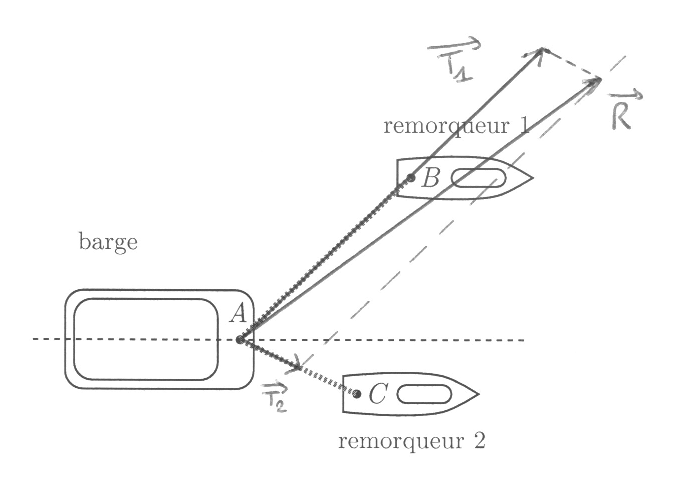
\includegraphics[width=.8\linewidth]{./exerciceBargeCorr}   

\item Sur le graphique, la résultante $\vect{R}$ est représentée par 7,5\,cm. Son intensité est donc de 90\,kN.
\end{enumerate}
\end{corrige}


% ex DOI


 \serie{Diagramme objets--interactions}

Pour les exercices \RefExercice{doiFirst} à \RefExercice{doiLast} établir un diagramme objets--interactions et en déduire le nombre de forces appliquées au système (le système étudié est indiqué en dessous de la figure).

\begin{exercice}\ExerciceRefMethode{methodeDOI}
\label{doiFirst}
\begin{center}
    \includegraphics[width=.2\linewidth]{./pendule}  
    
    Bille
\end{center}
\end{exercice}

\begin{corrige}
Bille

\begin{center}
    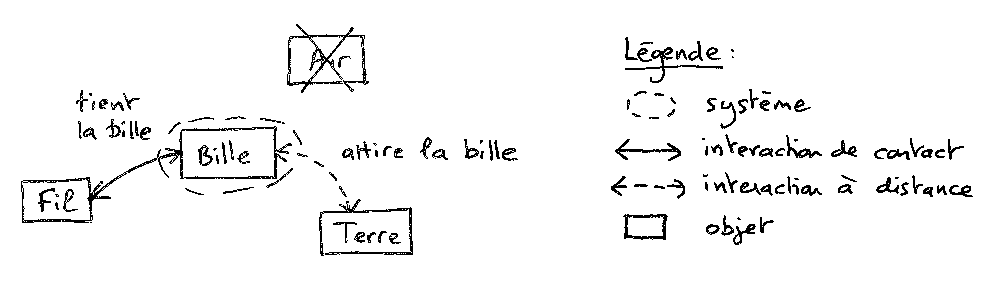
\includegraphics[width=\linewidth]{./doiBille}  
\end{center}
Il y a deux interactions dans le DOI donc le système est soumis à deux forces : l'attraction gravitationnelle de la Terre et la force de tension du fil qui retient la bille. L'action de l'air est négligée car la bille n'est pas en mouvement et sa masse volumique est bien plus grande que celle de l'air.
\end{corrige}

\begin{exercice}
\begin{center}
    \includegraphics[width=.4\linewidth]{./patinGlace}   
    
    Patineuse qui avance lentement
\end{center}
\end{exercice}

\begin{corrige}
Patineuse

\begin{center}
    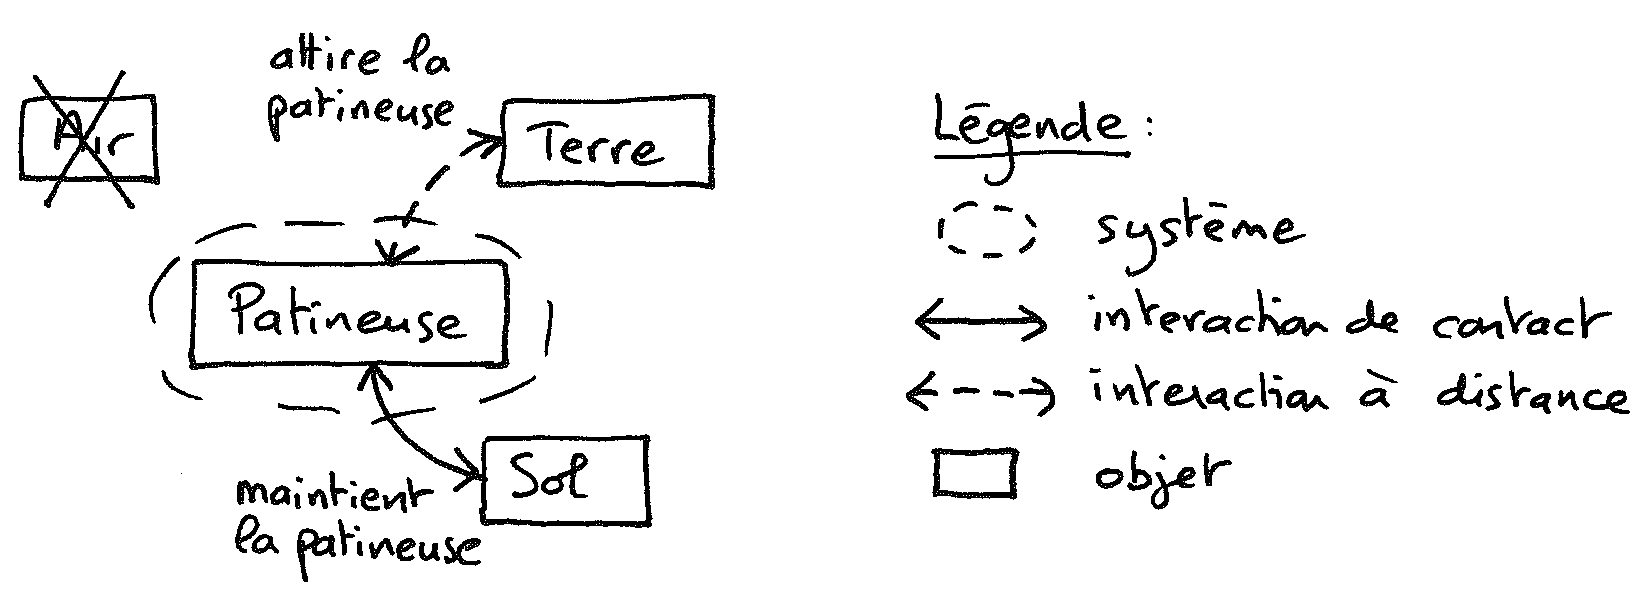
\includegraphics[width=\linewidth]{./doiPatineuse}  
\end{center}
Il y a deux interactions dans le DOI donc le système est soumis à deux forces : l'attraction gravitationnelle de la Terre et la réaction du support. L'action de l'air est négligée car la patineuse avance lentement et sa masse volumique est bien plus grande que celle de l'air.
\end{corrige}

\begin{exercice}
\begin{center}
    \includegraphics[width=.5\linewidth]{./voiturePente} 
    
    Voiture arrêtée dans une pente
\end{center}
\end{exercice}

\begin{corrige}
Voiture

\begin{center}
    %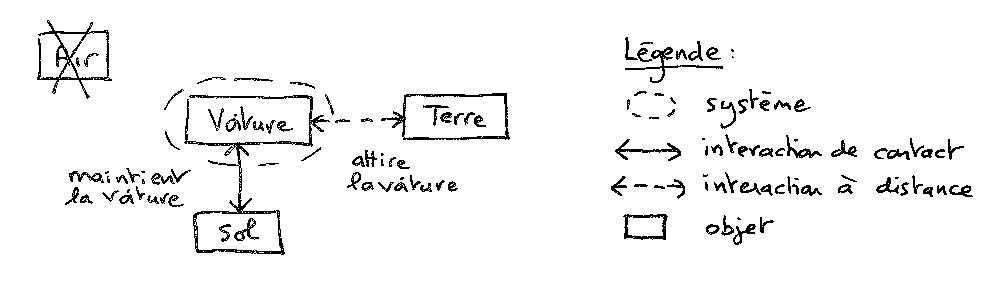
\includegraphics[width=\linewidth]{./doiVoiture}  
\end{center}
\end{corrige}

\begin{exercice}
\begin{center}
    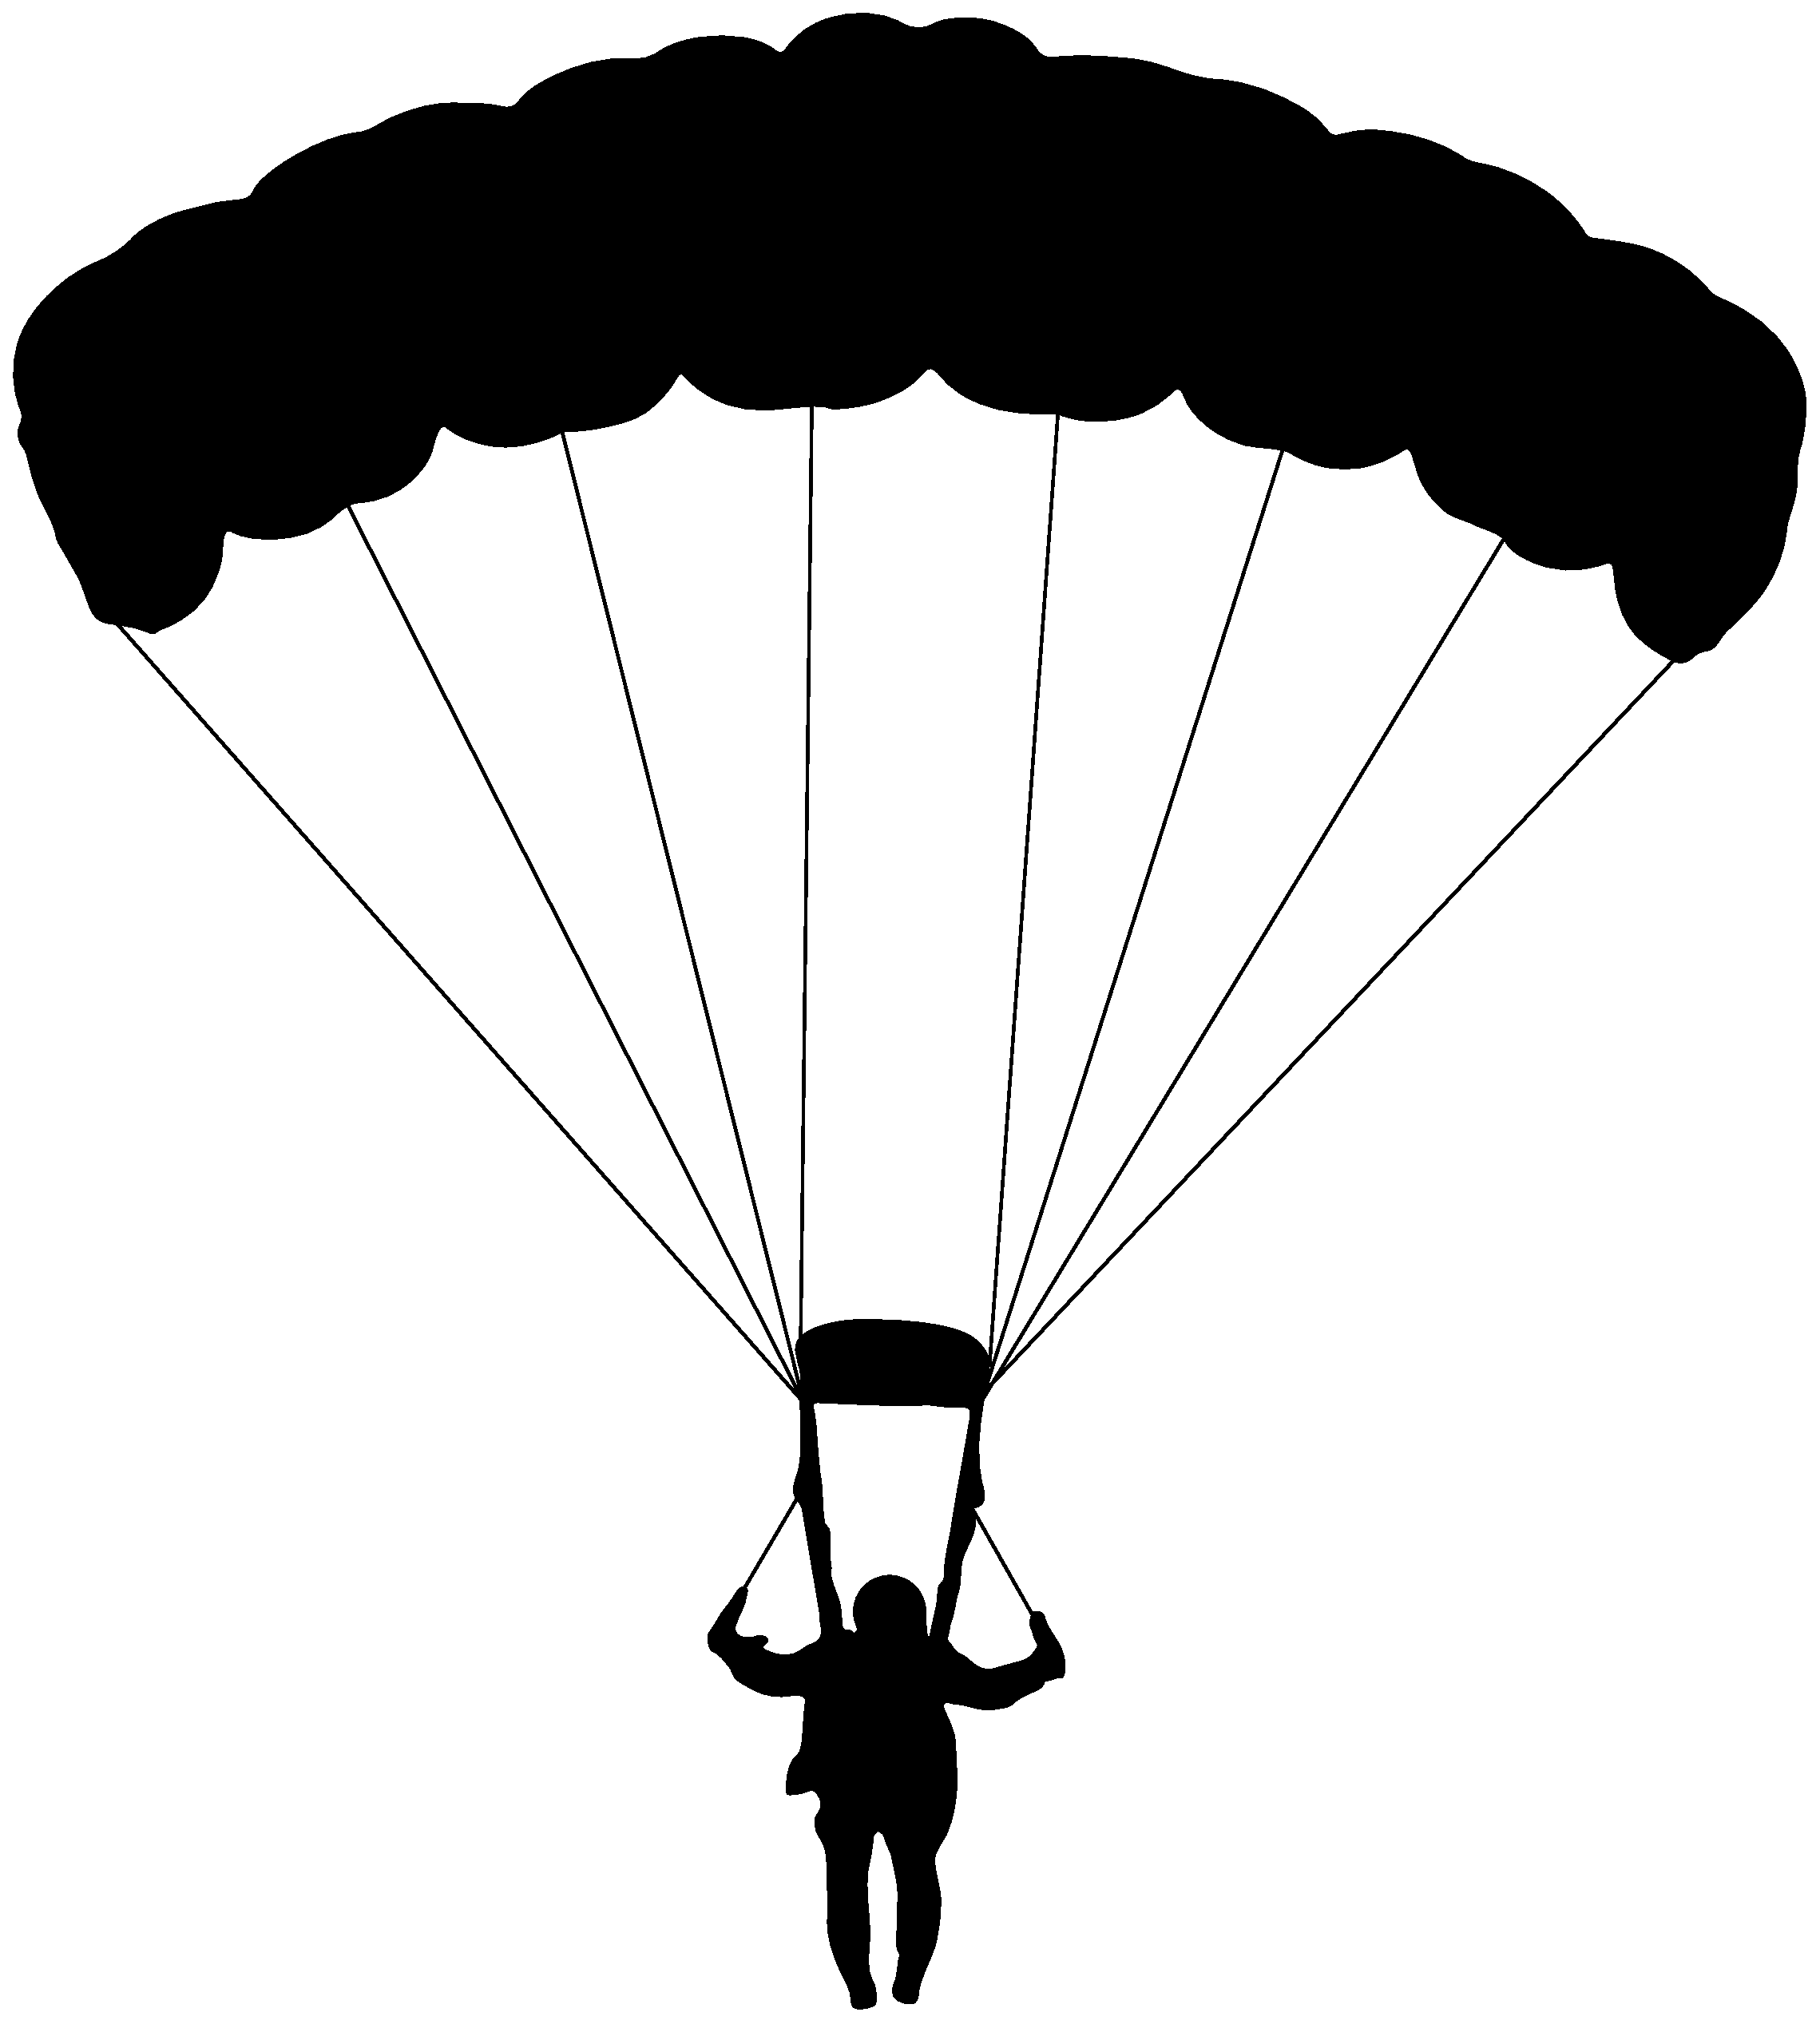
\includegraphics[width=.2\linewidth]{./parachute} 
    
    Parachutiste et son matériel
\end{center}
\end{exercice}



\begin{exercice}
\begin{center}
    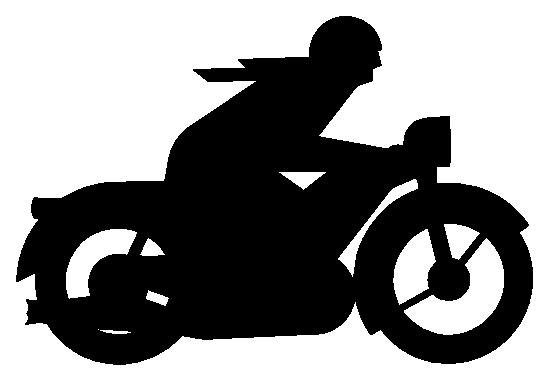
\includegraphics[width=.3\linewidth]{./moto}
    
    Moto qui roule vite
\end{center}
\end{exercice}



\begin{exercice}\label{doiLast}
\begin{center}
    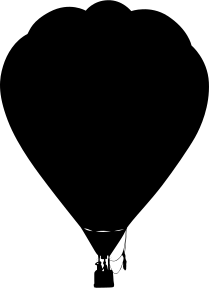
\includegraphics[width=.2\linewidth]{./montgolfiere}
    
    Montgolfière qui se déplace avec la masse d'air
\end{center}
\end{exercice}


























































